\documentclass{article}
\title{Notes for: Algorithms for Inverse Reinforcement Learning}
\author{-- \thanks{paper: https://ai.stanford.edu/~ang/papers/icml00-irl.pdf}}
\date{\today}
\usepackage{graphicx}

\begin{document}
    \maketitle
    
    \section{High Level and Motivation}

    \subsection{Problem}
    
    \begin{itemize}
        \item Normal reinforcement learning is the process of extracting an optimal policy for a given reward function in an environment.
        \item Inverse reinforcement learning is the process of extracting a reward function from an environment given observed optimal behavior.
    \end{itemize}
    
    \subsection{Example}
    You are able to observe an agent as it tackles the Mountain Car problem:
    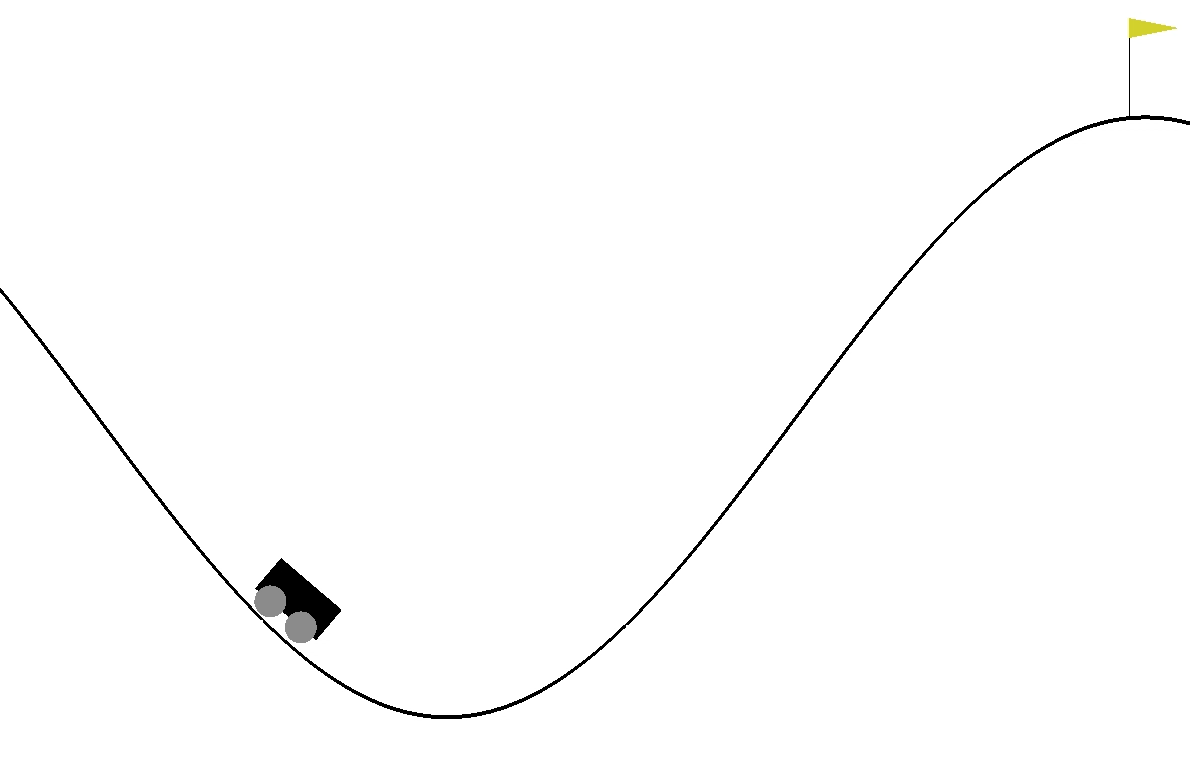
\includegraphics[width=10cm]{fig1.png}

    \section{Medium Level}

    \section{Low Level}

\end{document}